\documentclass[paper]{IEEEtran}
\IEEEoverridecommandlockouts
% The preceding line is only needed to identify funding in the first footnote. If that is unneeded, please comment it out.
\usepackage[english]{babel}
\usepackage[utf8x]{inputenc}
\usepackage{amsmath}
\usepackage{graphicx}
\usepackage[colorinlistoftodos]{todonotes}
\usepackage{gensymb} % this could be problem
\usepackage{float}
\usepackage{fancyref}
\usepackage{subcaption}
\usepackage{amssymb}

\usepackage{pythonhighlight}

\usepackage{xspace}

\newcommand\nd{\textsuperscript{nd}\xspace}
\newcommand\rd{\textsuperscript{rd}\xspace}
\newcommand\nth{\textsuperscript{th}\xspace} %\th is taken already


\usepackage{xcolor}
\usepackage{listings}

\usepackage{fancyhdr}

\usepackage{karnaugh-map}

\definecolor{mGreen}{rgb}{0,0.6,0} % for python
\definecolor{mGray}{rgb}{0.5,0.5,0.5}
\definecolor{mPurple}{rgb}{0.58,0,0.82}


\definecolor{mygreen}{RGB}{28,172,0} % color values Red, Green, Blue for matlab
\definecolor{mylilas}{RGB}{170,55,241}

\lstdefinestyle{CStyle}{
    commentstyle=\color{mGreen},
    keywordstyle=\color{magenta},
    numberstyle=\tiny\color{mGray},
    stringstyle=\color{mPurple},
    basicstyle=\footnotesize,
    breakatwhitespace=false,         
    breaklines=true,                 
    captionpos=b,                    
    keepspaces=true,                 
    numbers=left,                    
    numbersep=5pt,                  
    showspaces=false,                
    showstringspaces=false,
    showtabs=false,                  
    tabsize=2,
    language=C
}


\lstset{language=Matlab,%
    %basicstyle=\color{red},
    breaklines=true,%
    morekeywords={matlab2tikz},
    keywordstyle=\color{blue},%
    morekeywords=[2]{1}, keywordstyle=[2]{\color{black}},
    identifierstyle=\color{black},%
    stringstyle=\color{mylilas},
    commentstyle=\color{mygreen},%
    showstringspaces=false,%without this there will be a symbol in the places where there is a space
    numbers=left,%
    numberstyle={\tiny \color{black}},% size of the numbers
    numbersep=9pt, % this defines how far the numbers are from the text
    emph=[1]{for,end,break},emphstyle=[1]\color{red}, %some words to emphasise
    %emph=[2]{word1,word2}, emphstyle=[2]{style},    
}



\makeatletter
\renewcommand\paragraph{\@startsection{paragraph}{4}{\z@}%
            {-2.5ex\@plus -1ex \@minus -.25ex}%
            {1.25ex \@plus .25ex}%
            {\normalfont\normalsize\bfseries}}
\makeatother
\setcounter{secnumdepth}{4} % how many sectioning levels to assign numbers to
\setcounter{tocdepth}{4}    % how many sectioning levels to show in ToC



\begin{document}

\title{EE314 Digital Electronics Laboratory\\
2017-2018 Spring Term Project Proposal Report
}


\author{

\IEEEauthorblockN{1\textsuperscript{st} Halil TEMURTAS}
\IEEEauthorblockA{\textit{2094522} }
\textit{halil.temurtas@metu.edu.tr}

\and

\IEEEauthorblockN{2\textsuperscript{nd} Erdem TUNA}
\IEEEauthorblockA{\textit{2167419} }
\textit{erdem.tuna@metu.edu.tr}


}

\maketitle

\begin{abstract}

The project 

\end{abstract}

\begin{IEEEkeywords}
The, laboratory , project
\end{IEEEkeywords}

\section{Introduction}
\- \indent
	In this project, our aim is to design a oscilloscope.


\section{Project}
\- \indent


\begin{figure}[h!]
	\setlength{\unitlength}{\textwidth}
	\center 
	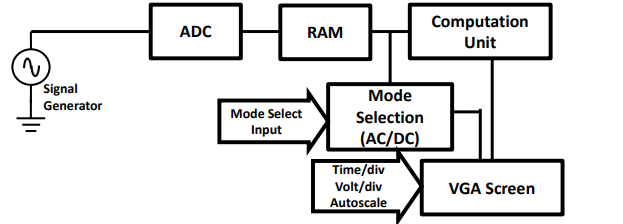
\includegraphics[width=0.47\textwidth]{block_diagram}
	\caption{\label{fig:block_diagram}The Block Diagram of the project}
\end{figure}

	 \textit{Figure~\ref{fig:block_diagram}}    

	
%\begin{figure}[h!]
%	\centering
%	\begin{subfigure}{.48\textwidth}
%		\centering
%		\includegraphics[width=1\linewidth]{scope_28_SimResult}
		%\caption{Theoretical Output of VCO.}
		%\label{fig:VCOFor1kHzTheoretical}
%	\end{subfigure}%
%	\newline
%	\begin{subfigure}{.48\textwidth}
%		\centering
%		\includegraphics[width=1\linewidth]{scope_28}
		%\caption{Practical Output of VCO.}
		%\label{fig:VCOFor1kHzPractical}
%	\end{subfigure}
	%\caption{VCO Outputs for 1kHz.}
%	\label{fig:VCOFor1kHz}
%\end{figure}

\subsection{ADC} \- \indent
		This module quantizes the analog input data. The hardware used is LTC2308 that is built into the FPGA. The Altera provides an example code regarding the use of the built-in ADC\cite{b1}. By evaluating the provided functionalities of this example with the help of a MsC project \cite{b2}, a code is written in Verilog HDL and in Qsys environment. 

\subsection{RAM} \- \indent

\subsection{Computation Unit} \- \indent
	Computation unit is the unit responsible for all kinds of mathematical calculation of the project. This Unit can be considered as a brain of the project. 

\subsection{Mode Selection (AC/DC)} \- \indent
	One slide switch will be assigned to retrieve the desired mode information from the user. Based on this information, screen will display the input signal either with the DC offset or without the DC offset.

\subsubsection{AC Mode} \- \indent
	In AC Mode operation of the oscilloscope, the DC offset voltage is removed from the input voltage before it is reflected to the VGA monitor. For that Computation Unit will be used to extract offset information from stored data.

\subsubsection{DC Mode} \- \indent
	In DC Mode operation of the oscilloscope, the DC offset voltage is untouched from the stored data of the input voltage. The stored data is reflected directly to the VGA monitor. 
	

\subsection{VGA Screen} \- \indent
	VGA is a widely used standard in video industry for the transmission of video signals from a computer or microprocessor into a monitor or TV. Each 640x480 image is called a ‘frame’ and each frame contains 480 lines which are made up of 640 pixels. We will use a standard LCD VGA Monitor as a display for our FPGA Oscilloscope. We will build a controller module for this part called VGA Controller. 
	

\subsubsection{VGA Controller} \- \indent

	The VGA controller combines the data drom RAM and Computation Unit to create a signal that can be displayed on the VGA monitor. Each of the RAM Modules contains an image that is ready for display on the screen. However, the data must be positioned relative to each other and combined. Also this module performs once a second as desired in the project requirements. The VGA controller also gets data from different data inputs such as Time/div and Voltage/div in order to reflect the waveform as user requires.

\subsubsection{Time/div Input} \- \indent
	
	This module will supply an input data for the VGA controller for user preferences. Two push buttons will be assigned for the Time/div inputs that can be considered as Time+/div and Time-/div. As user pushes to Time+/div button, the time scale will be larger than the previous value. Similarly, as the user pushes to Time-/div button, the time scale will be smaller than the previous value. According to user preferences, this module allows user to see wider or narrower parts of input waveform.
	  
\subsubsection{Voltage/div Input} \- \indent

	This module will supply an input data for the VGA controller for user preferences. Two push buttons will be assigned for the Voltage/div inputs that can be considered as Voltage+/div and Voltage-/div. As user pushes to Voltage+/div button, the voltage scale will be larger than the previous value. Similarly, as the user pushes to Voltage-/div button, the voltage scale will be smaller than the previous value. According to user preferences, this module allows user to fit the voltage waveform to the screen.
	
\subsubsection{Autoscale Input} \- \indent

	This module will also supply an input data for the VGA controller for user preferences. Since we are planning to use all push buttons for other modules. One slide switch will be assigned to this module. As the user triggers the button, this module will scale the waveform for the display such that it fits the display best.

	
	
\section{Conclusion}
\- \indent
	Conclusion
	
	

\begin{thebibliography}{00}
\bibitem{b1} “De1-Soc CD.” [Online]. Available: http://download.terasic.com/downloads/cd-rom/de1-soc/DE1-SoC\_v.5.0.1\_HWrevF\_SystemCD.zip. [Accessed: 21-May-2018].
\bibitem{b2} “Digital Scope Implemented on Altera DE1-SoC.” [Online]. Available: https://people.ece.cornell.edu/land/courses/eceprojectsland/STUDENTPROJ/2015to2016/hj424/hj424\_report\_201605191237.pdf. [Accessed: 21-May-2018].
%\bibitem{b3} “2N7000 Datasheet.” [Online]. Available: https://www.onsemi.com/pub/Collateral/2N7000-D.PDF. [Accessed: 20-Jan-2018].
%\bibitem{b4} “LF353 Datasheet.” [Online]. Available: http://www.falstad.com/circuit/e-vco.html.

%\bibitem{b6} Y. Yorozu, M. Hirano, K. Oka, and Y. Tagawa, ``Electron spectroscopy studies on magneto-optical media and plastic substrate interface,'' IEEE Transl. J. Magn. Japan, vol. 2, pp. 740--741, August 1987 [Digests 9th Annual Conf. Magnetics Japan, p. 301, 1982].
%\bibitem{b7} M. Young, The Technical Writer's Handbook. Mill Valley, CA: University Science, 1989.
\end{thebibliography}




\end{document}